% Options for packages loaded elsewhere
\PassOptionsToPackage{unicode}{hyperref}
\PassOptionsToPackage{hyphens}{url}
%
\documentclass[
]{article}
\usepackage{lmodern}
\usepackage{amssymb,amsmath}
\usepackage{ifxetex,ifluatex}
\ifnum 0\ifxetex 1\fi\ifluatex 1\fi=0 % if pdftex
  \usepackage[T1]{fontenc}
  \usepackage[utf8]{inputenc}
  \usepackage{textcomp} % provide euro and other symbols
\else % if luatex or xetex
  \usepackage{unicode-math}
  \defaultfontfeatures{Scale=MatchLowercase}
  \defaultfontfeatures[\rmfamily]{Ligatures=TeX,Scale=1}
\fi
% Use upquote if available, for straight quotes in verbatim environments
\IfFileExists{upquote.sty}{\usepackage{upquote}}{}
\IfFileExists{microtype.sty}{% use microtype if available
  \usepackage[]{microtype}
  \UseMicrotypeSet[protrusion]{basicmath} % disable protrusion for tt fonts
}{}
\makeatletter
\@ifundefined{KOMAClassName}{% if non-KOMA class
  \IfFileExists{parskip.sty}{%
    \usepackage{parskip}
  }{% else
    \setlength{\parindent}{0pt}
    \setlength{\parskip}{6pt plus 2pt minus 1pt}}
}{% if KOMA class
  \KOMAoptions{parskip=half}}
\makeatother
\usepackage{xcolor}
\IfFileExists{xurl.sty}{\usepackage{xurl}}{} % add URL line breaks if available
\IfFileExists{bookmark.sty}{\usepackage{bookmark}}{\usepackage{hyperref}}
\hypersetup{
  pdftitle={GenoSee Business Model},
  pdfauthor={Omer Perach},
  hidelinks,
  pdfcreator={LaTeX via pandoc}}
\urlstyle{same} % disable monospaced font for URLs
\usepackage[margin=1in]{geometry}
\usepackage{color}
\usepackage{fancyvrb}
\newcommand{\VerbBar}{|}
\newcommand{\VERB}{\Verb[commandchars=\\\{\}]}
\DefineVerbatimEnvironment{Highlighting}{Verbatim}{commandchars=\\\{\}}
% Add ',fontsize=\small' for more characters per line
\usepackage{framed}
\definecolor{shadecolor}{RGB}{248,248,248}
\newenvironment{Shaded}{\begin{snugshade}}{\end{snugshade}}
\newcommand{\AlertTok}[1]{\textcolor[rgb]{0.94,0.16,0.16}{#1}}
\newcommand{\AnnotationTok}[1]{\textcolor[rgb]{0.56,0.35,0.01}{\textbf{\textit{#1}}}}
\newcommand{\AttributeTok}[1]{\textcolor[rgb]{0.77,0.63,0.00}{#1}}
\newcommand{\BaseNTok}[1]{\textcolor[rgb]{0.00,0.00,0.81}{#1}}
\newcommand{\BuiltInTok}[1]{#1}
\newcommand{\CharTok}[1]{\textcolor[rgb]{0.31,0.60,0.02}{#1}}
\newcommand{\CommentTok}[1]{\textcolor[rgb]{0.56,0.35,0.01}{\textit{#1}}}
\newcommand{\CommentVarTok}[1]{\textcolor[rgb]{0.56,0.35,0.01}{\textbf{\textit{#1}}}}
\newcommand{\ConstantTok}[1]{\textcolor[rgb]{0.00,0.00,0.00}{#1}}
\newcommand{\ControlFlowTok}[1]{\textcolor[rgb]{0.13,0.29,0.53}{\textbf{#1}}}
\newcommand{\DataTypeTok}[1]{\textcolor[rgb]{0.13,0.29,0.53}{#1}}
\newcommand{\DecValTok}[1]{\textcolor[rgb]{0.00,0.00,0.81}{#1}}
\newcommand{\DocumentationTok}[1]{\textcolor[rgb]{0.56,0.35,0.01}{\textbf{\textit{#1}}}}
\newcommand{\ErrorTok}[1]{\textcolor[rgb]{0.64,0.00,0.00}{\textbf{#1}}}
\newcommand{\ExtensionTok}[1]{#1}
\newcommand{\FloatTok}[1]{\textcolor[rgb]{0.00,0.00,0.81}{#1}}
\newcommand{\FunctionTok}[1]{\textcolor[rgb]{0.00,0.00,0.00}{#1}}
\newcommand{\ImportTok}[1]{#1}
\newcommand{\InformationTok}[1]{\textcolor[rgb]{0.56,0.35,0.01}{\textbf{\textit{#1}}}}
\newcommand{\KeywordTok}[1]{\textcolor[rgb]{0.13,0.29,0.53}{\textbf{#1}}}
\newcommand{\NormalTok}[1]{#1}
\newcommand{\OperatorTok}[1]{\textcolor[rgb]{0.81,0.36,0.00}{\textbf{#1}}}
\newcommand{\OtherTok}[1]{\textcolor[rgb]{0.56,0.35,0.01}{#1}}
\newcommand{\PreprocessorTok}[1]{\textcolor[rgb]{0.56,0.35,0.01}{\textit{#1}}}
\newcommand{\RegionMarkerTok}[1]{#1}
\newcommand{\SpecialCharTok}[1]{\textcolor[rgb]{0.00,0.00,0.00}{#1}}
\newcommand{\SpecialStringTok}[1]{\textcolor[rgb]{0.31,0.60,0.02}{#1}}
\newcommand{\StringTok}[1]{\textcolor[rgb]{0.31,0.60,0.02}{#1}}
\newcommand{\VariableTok}[1]{\textcolor[rgb]{0.00,0.00,0.00}{#1}}
\newcommand{\VerbatimStringTok}[1]{\textcolor[rgb]{0.31,0.60,0.02}{#1}}
\newcommand{\WarningTok}[1]{\textcolor[rgb]{0.56,0.35,0.01}{\textbf{\textit{#1}}}}
\usepackage{graphicx,grffile}
\makeatletter
\def\maxwidth{\ifdim\Gin@nat@width>\linewidth\linewidth\else\Gin@nat@width\fi}
\def\maxheight{\ifdim\Gin@nat@height>\textheight\textheight\else\Gin@nat@height\fi}
\makeatother
% Scale images if necessary, so that they will not overflow the page
% margins by default, and it is still possible to overwrite the defaults
% using explicit options in \includegraphics[width, height, ...]{}
\setkeys{Gin}{width=\maxwidth,height=\maxheight,keepaspectratio}
% Set default figure placement to htbp
\makeatletter
\def\fps@figure{htbp}
\makeatother
\setlength{\emergencystretch}{3em} % prevent overfull lines
\providecommand{\tightlist}{%
  \setlength{\itemsep}{0pt}\setlength{\parskip}{0pt}}
\setcounter{secnumdepth}{-\maxdimen} % remove section numbering

\title{GenoSee Business Model}
\author{Omer Perach}
\date{2020-07-30}

\begin{document}
\maketitle

\hypertarget{executive-summary}{%
\subsection{Executive Summary}\label{executive-summary}}

Wordlwide climate change and decrease in arable lands and lands under
permanent crops constitute a major concern for future food safety.
Private and goverment based breeding programs working constantly to
develop elite crops in order to meet the future demand to feed 10
billion people by 2050. Under these constraints, to meet the rising
demand for food, agricultural production must increase by an estimated
50\% without greatly increasing water usage or expanding the total land
area dedicated to agriculture. The era of data enable us to make
processes highly effieciet for companies and organisations. This is also
true for the plant breeding industry, huge amount of data is recorded
and collected - genotype, phenotype, environmental etc. Before inferring
and analyzing the data, it should be transformed into findable,
available, identifiable, reusable database. GenoSee is a one stop shop
for all the breeding program associates which let them focus in
achieving their goal - developing elite crops - while letting GenoSee
handle the data related work. GenoSee estimate that it will reach 50
paying breeding programs worldwide during the next four years. We are
asking for \textbf{\$1M} dollars for the first phase of development and
\textbf{\$500K} for the second phase of devlopment. Following our
assumptions we calculte a potential positive \textbf{NPV}.

\hypertarget{assumptions}{%
\subsection{Assumptions}\label{assumptions}}

\begin{enumerate}
\def\labelenumi{\arabic{enumi}.}
\tightlist
\item
  Thousands of open plant breeding programs worldwide.
\item
  Phase 1 - one year to MVP and reaching first customers.
\item
  Phase 2 - one year for improvement and growth.
\item
  We will look on the next 7 years.
\item
  Tax rate 38\%.
\item
  Discount rate 12\%.
\item
  Depreciation 4 years straight line.
\item
  During the next four years we will reach 50 breeding programs (to our
  opinion it is a conservative aproach).
\item
  GenoSee will charge 15000 dollars for building the database abd
  additional 300 dollars per user monthly.
\item
  GenoSee estimating average of 10 users per breeding program.
\end{enumerate}

\hypertarget{capex-block}{%
\subsection{CAPEX Block}\label{capex-block}}

We will start by creating a depreciation matrix for the capital
investment of the company. We will assume 4 years straight line
depreciation that will taken into account only until it can be applied
against taxable profit .

\begin{Shaded}
\begin{Highlighting}[]
\NormalTok{kHorizon<-}\DecValTok{7} \CommentTok{# The model Horizon}
\NormalTok{year<-}\DecValTok{1}\OperatorTok{:}\NormalTok{kHorizon }\CommentTok{# A sequence to represent the horizon years}
\NormalTok{kTaxRate<-}\DecValTok{38} \CommentTok{# Tax percentage}
\NormalTok{kDiscountrate<-}\DecValTok{12} \CommentTok{# Discount rate percentage per year for NPV calculations.}
\NormalTok{kDeprPer<-}\DecValTok{4} \CommentTok{#month, the deprciation sheduale for the capital}
\NormalTok{p1.dur<-}\DecValTok{1} \CommentTok{#Duration phase one in year}
\NormalTok{p2.dur<-}\DecValTok{1} \CommentTok{#Duration phase 2 in year}
\NormalTok{p1.capex<-}\DecValTok{1000000} \CommentTok{#Investment for phase 1.}
\NormalTok{p2.capex<-}\DecValTok{500000} \CommentTok{#Investment phase 2.}
\NormalTok{maint.capex<-}\DecValTok{0} \CommentTok{# Additional parameter nit used.}
\NormalTok{time.to.peak.sales<-}\DecValTok{3} \CommentTok{#Time to reach 100 breedings programs.}
\NormalTok{mkt.demand<-}\DecValTok{50} \CommentTok{# Market demand after 4 years.}
\NormalTok{phase <-}\StringTok{ }\NormalTok{(year }\OperatorTok{<=}\StringTok{ }\NormalTok{p1.dur) }\OperatorTok{*}\StringTok{ }\DecValTok{1} \OperatorTok{+}
\NormalTok{(year }\OperatorTok{>}\StringTok{ }\NormalTok{p1.dur }\OperatorTok{&}\StringTok{ }\NormalTok{year }\OperatorTok{<=}\StringTok{ }\NormalTok{(p1.dur }\OperatorTok{+}\StringTok{ }\NormalTok{p2.dur)) }\OperatorTok{*}\StringTok{ }\DecValTok{2} \OperatorTok{+}
\NormalTok{(year }\OperatorTok{>}\StringTok{ }\NormalTok{(p1.dur }\OperatorTok{+}\StringTok{ }\NormalTok{p2.dur)) }\OperatorTok{*}\StringTok{ }\DecValTok{3}
\NormalTok{capex<-(phase}\OperatorTok{==}\DecValTok{1}\NormalTok{)}\OperatorTok{*}\NormalTok{p1.capex}\OperatorTok{/}\NormalTok{p1.dur}\OperatorTok{+}\NormalTok{(phase}\OperatorTok{==}\DecValTok{2}\NormalTok{)}\OperatorTok{*}\NormalTok{p2.capex}\OperatorTok{/}\NormalTok{p2.dur}\OperatorTok{+}\NormalTok{(phase}\OperatorTok{==}\DecValTok{3}\NormalTok{)}\OperatorTok{*}\NormalTok{maint.capex}
\NormalTok{depr.matrix <-}
\KeywordTok{t}\NormalTok{(}\KeywordTok{sapply}\NormalTok{(year, }\ControlFlowTok{function}\NormalTok{(y)}
\KeywordTok{ifelse}\NormalTok{(y }\OperatorTok{<=}\StringTok{ }\NormalTok{p1.dur }\OperatorTok{&}\StringTok{ }\NormalTok{year }\OperatorTok{>}\StringTok{ }\DecValTok{0}\NormalTok{,}\DecValTok{0}\NormalTok{,}\KeywordTok{ifelse}\NormalTok{(}
\NormalTok{y }\OperatorTok{==}\StringTok{ }\NormalTok{(p1.dur }\OperatorTok{+}\StringTok{ }\DecValTok{1}\NormalTok{) }\OperatorTok{&}\StringTok{ }\NormalTok{year }\OperatorTok{<}\StringTok{ }\NormalTok{y }\OperatorTok{+}\StringTok{ }\NormalTok{kDeprPer }\OperatorTok{&}\StringTok{ }\NormalTok{year }\OperatorTok{>=}\StringTok{ }\NormalTok{y,}
\NormalTok{p1.capex }\OperatorTok{/}\StringTok{ }\NormalTok{kDeprPer,}
\KeywordTok{ifelse}\NormalTok{((year }\OperatorTok{>=}\StringTok{ }\NormalTok{y) }\OperatorTok{&}\StringTok{ }\NormalTok{(year }\OperatorTok{<}\StringTok{ }\NormalTok{(y }\OperatorTok{+}\StringTok{ }\NormalTok{kDeprPer)),}
\NormalTok{capex[y }\OperatorTok{-}\StringTok{ }\DecValTok{1}\NormalTok{] }\OperatorTok{/}\StringTok{ }\NormalTok{kDeprPer, }\DecValTok{0}\NormalTok{)}
\NormalTok{)}
\NormalTok{)}
\NormalTok{)}
\NormalTok{)}
\NormalTok{depr.matrix}
\end{Highlighting}
\end{Shaded}

\begin{verbatim}
##      [,1]   [,2]   [,3]   [,4]   [,5]   [,6] [,7]
## [1,]    0      0      0      0      0      0    0
## [2,]    0 250000 250000 250000 250000      0    0
## [3,]    0      0 125000 125000 125000 125000    0
## [4,]    0      0      0      0      0      0    0
## [5,]    0      0      0      0      0      0    0
## [6,]    0      0      0      0      0      0    0
## [7,]    0      0      0      0      0      0    0
\end{verbatim}

\begin{Shaded}
\begin{Highlighting}[]
\NormalTok{depr<-}\KeywordTok{colSums}\NormalTok{(depr.matrix)}
\KeywordTok{plot}\NormalTok{(year,depr}\OperatorTok{/}\FloatTok{1e3}\NormalTok{,}\DataTypeTok{xlab=}\StringTok{"Year"}\NormalTok{,}\DataTypeTok{ylab=}\StringTok{"Depreciation[$000]"}\NormalTok{,}\DataTypeTok{type =}\StringTok{"b"}\NormalTok{ )}
\end{Highlighting}
\end{Shaded}

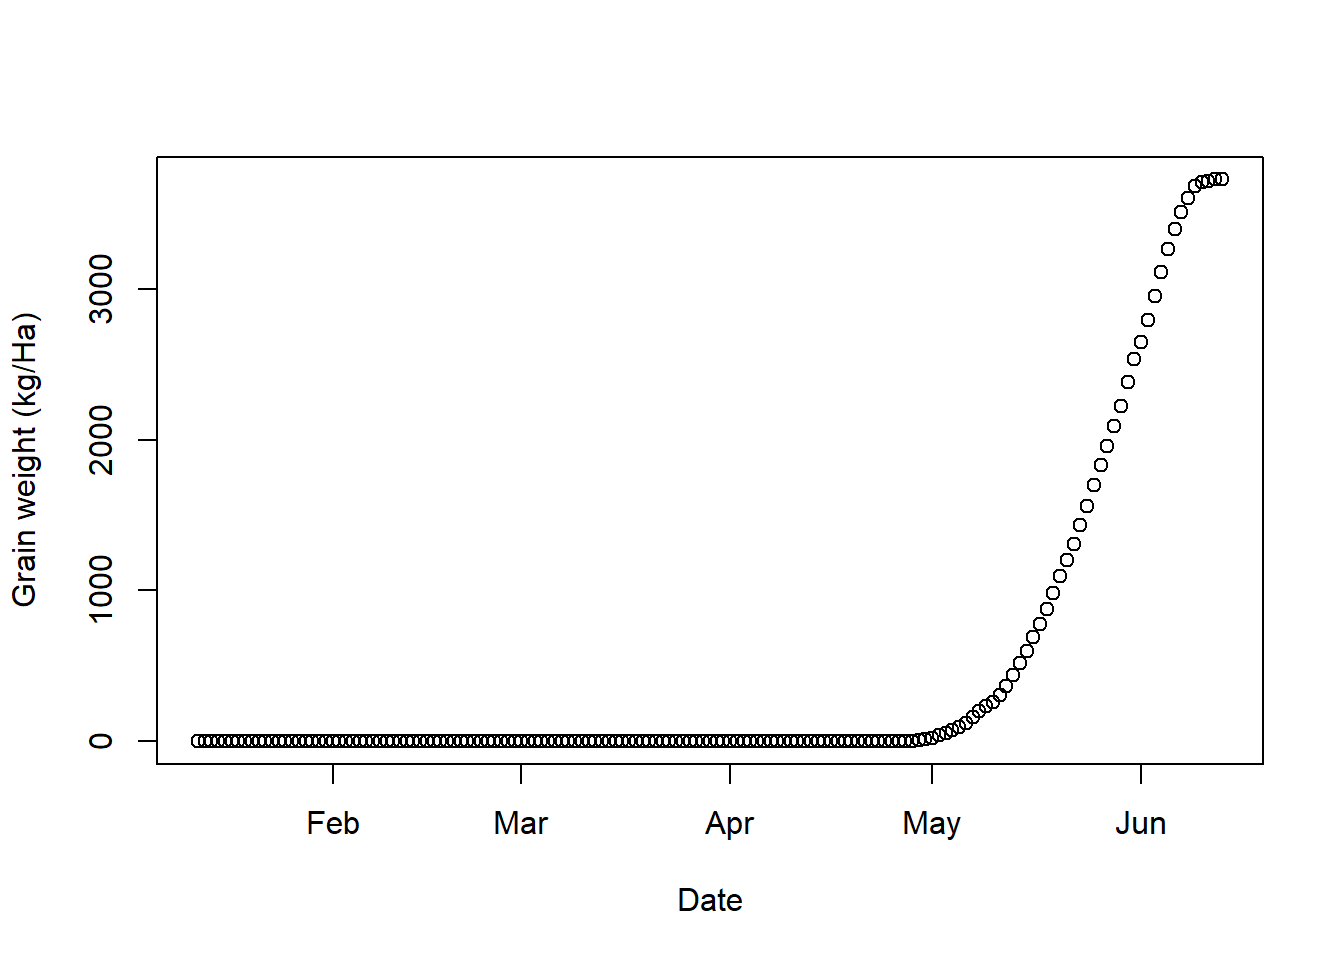
\includegraphics{2020-07-06-pre-seed-early-stage-saas-startup-business-modeling_files/figure-latex/unnamed-chunk-1-1.pdf}

\hypertarget{sales-and-revenue-block}{%
\subsection{Sales and Revenue Block}\label{sales-and-revenue-block}}

We assume that it will take us 3 years after end of phase 1 to reach 50
breeding programs worldwide. We will price (assumption) the software to
be 15000 dollars per year and additional subscription price per user of
300 dollars per month. We estimate that each program will have 5 users
by average.

\begin{Shaded}
\begin{Highlighting}[]
\NormalTok{mkt.adoption<-}\KeywordTok{pmin}\NormalTok{(}\KeywordTok{cumsum}\NormalTok{(phase}\OperatorTok{>}\DecValTok{1}\NormalTok{)}\OperatorTok{/}\NormalTok{time.to.peak.sales,}\DecValTok{1}\NormalTok{)}
\NormalTok{price.per.software.year<-}\DecValTok{15000}
\NormalTok{price.per.user<-}\DecValTok{300}
\NormalTok{average.users.per.program<-}\DecValTok{10}
\NormalTok{month.per.year<-}\DecValTok{12}
\NormalTok{user.arr<-price.per.user}\OperatorTok{*}\NormalTok{average.users.per.program}\OperatorTok{*}\NormalTok{month.per.year}
\NormalTok{price<-price.per.software.year}\OperatorTok{+}\NormalTok{user.arr}
\NormalTok{sales<-mkt.adoption}\OperatorTok{*}\NormalTok{mkt.demand}
\NormalTok{revenue<-sales}\OperatorTok{*}\NormalTok{price}
\KeywordTok{plot}\NormalTok{(year, revenue}\OperatorTok{/}\DecValTok{1000000}\NormalTok{,}
\DataTypeTok{xlab =} \StringTok{"Year"}\NormalTok{,}
\DataTypeTok{ylab =} \StringTok{"Sales [000,000 $]"}\NormalTok{,}
\DataTypeTok{type =} \StringTok{"b"}\NormalTok{)}
\end{Highlighting}
\end{Shaded}

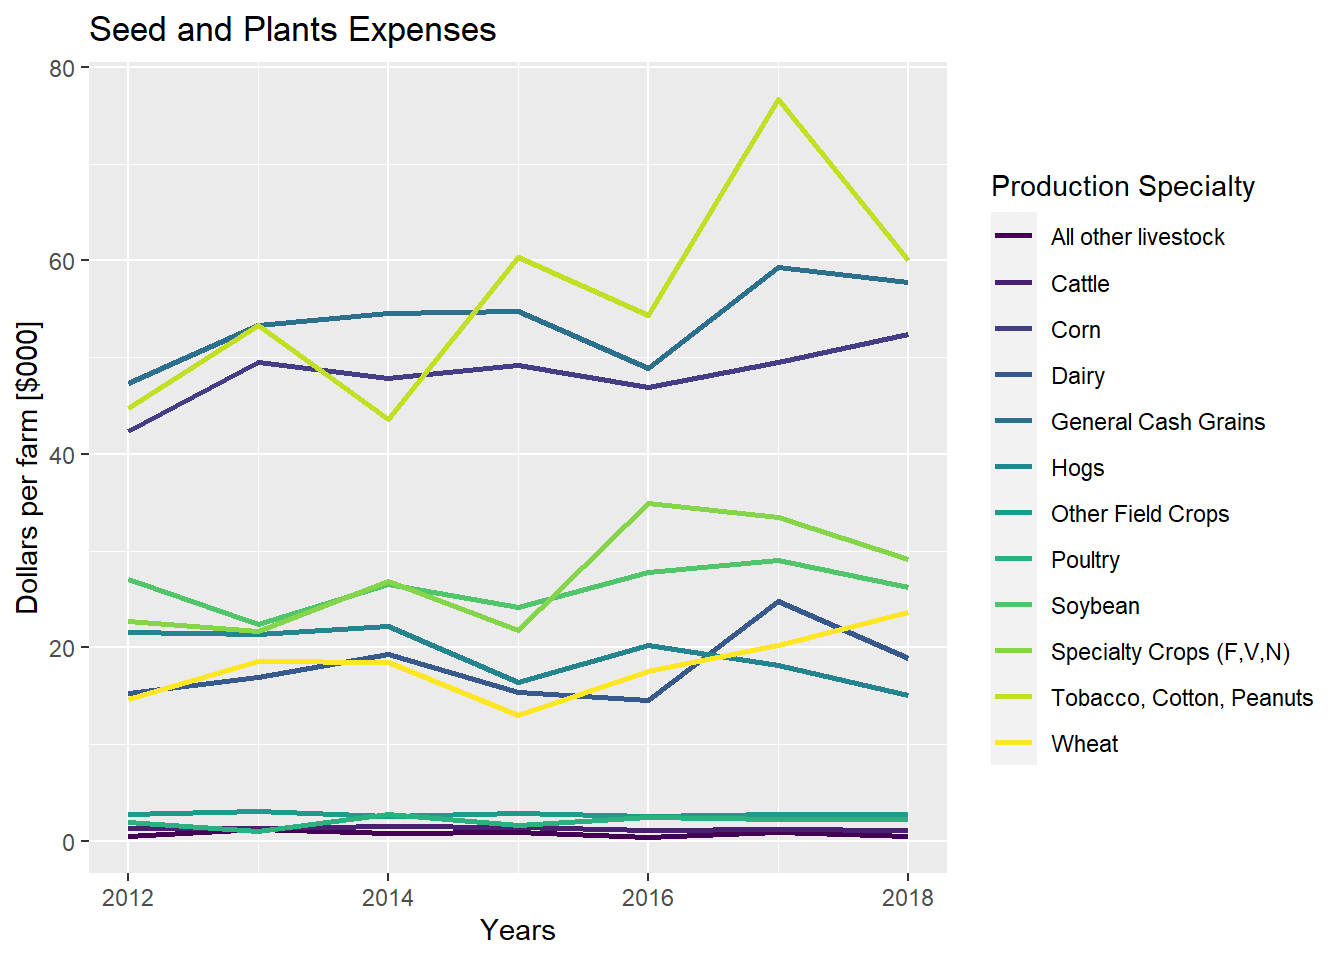
\includegraphics{2020-07-06-pre-seed-early-stage-saas-startup-business-modeling_files/figure-latex/unnamed-chunk-2-1.pdf}

\hypertarget{opex-block}{%
\subsection{OPEX Block}\label{opex-block}}

The OPEX include R\&D (research and development) and G\&S (general sales
and administrative) and is estimated to be 20\% of the revenue. The
operational cost will start only after phase 1.

\begin{Shaded}
\begin{Highlighting}[]
\NormalTok{opex<-revenue}\OperatorTok{*}\FloatTok{0.2}
\KeywordTok{plot}\NormalTok{(year, opex}\OperatorTok{/}\DecValTok{1000}\NormalTok{,}
\DataTypeTok{xlab =} \StringTok{"Year"}\NormalTok{,}
\DataTypeTok{ylab =} \StringTok{"Sales [000$]"}\NormalTok{,}
\DataTypeTok{type =} \StringTok{"b"}\NormalTok{)}
\end{Highlighting}
\end{Shaded}

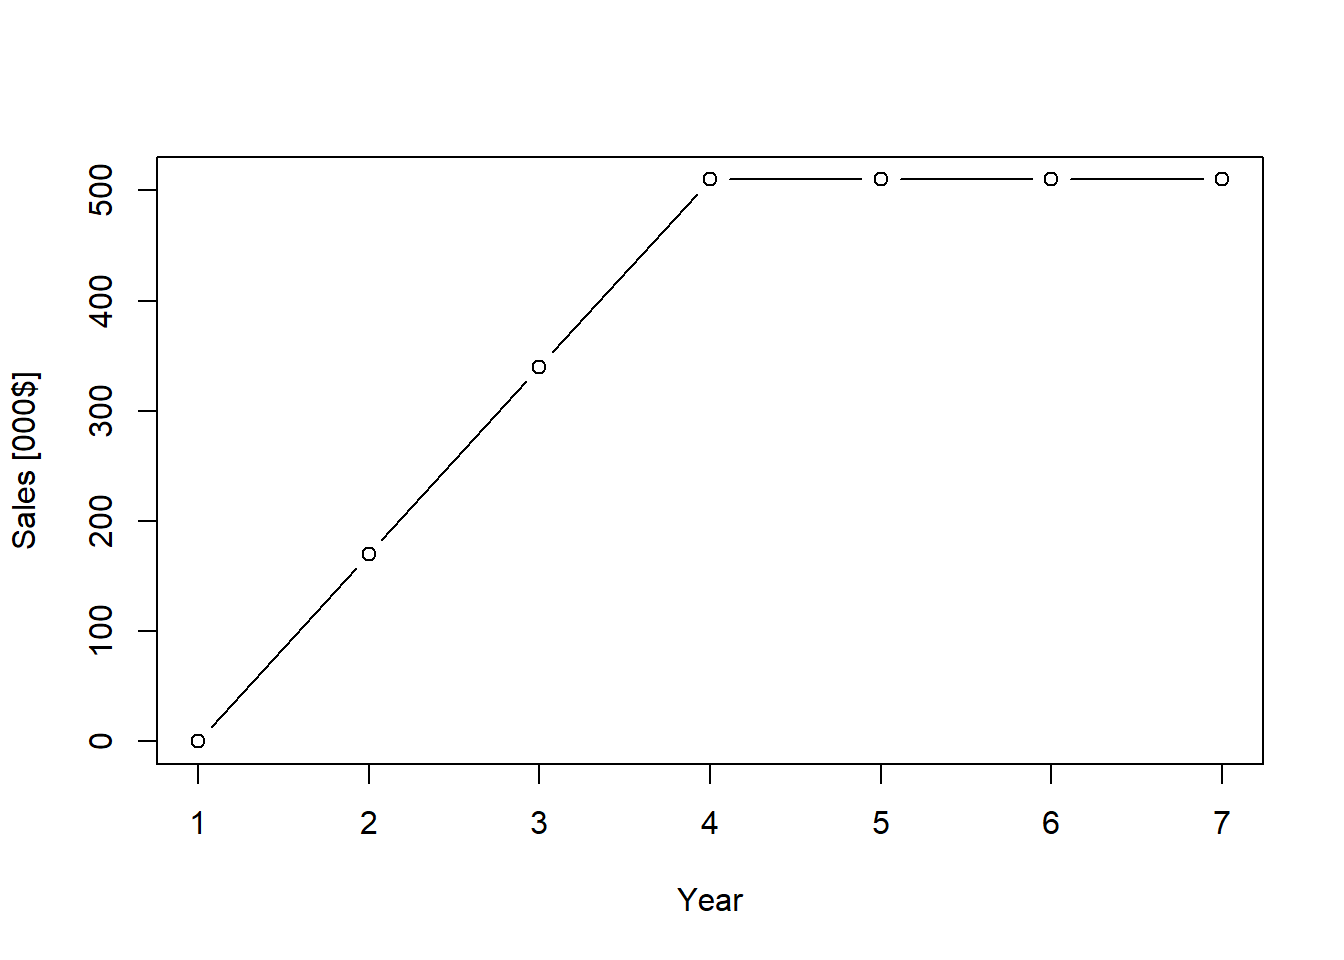
\includegraphics{2020-07-06-pre-seed-early-stage-saas-startup-business-modeling_files/figure-latex/unnamed-chunk-3-1.pdf}

\hypertarget{pro-forma-table}{%
\subsection{Pro Forma Table}\label{pro-forma-table}}

\begin{itemize}
\tightlist
\item
  Gross profit = revenue-OPEX
\item
  Operating profit before taxes = Gross profit - OPEX - depreciation
\item
  Operating profit after tax = operating profit before tax-tax
\item
  Cash flow = operating profit after tax + depreciation - CAPEX
\end{itemize}

\begin{Shaded}
\begin{Highlighting}[]
\NormalTok{gross.profit<-revenue}\OperatorTok{-}\NormalTok{opex}
\NormalTok{op.profit.before.tax<-gross.profit}\OperatorTok{-}\NormalTok{opex}\OperatorTok{-}\NormalTok{depr}
\NormalTok{tax<-op.profit.before.tax}\OperatorTok{*}\NormalTok{kTaxRate}\OperatorTok{/}\DecValTok{100}
\NormalTok{op.profit.after.tax<-op.profit.before.tax}\OperatorTok{-}\NormalTok{tax}
\NormalTok{cash.flow<-op.profit.after.tax}\OperatorTok{+}\NormalTok{depr}\OperatorTok{-}\NormalTok{capex}
\NormalTok{cum.cah.flow<-}\KeywordTok{cumsum}\NormalTok{(cash.flow)}
\end{Highlighting}
\end{Shaded}

\hypertarget{cumulative-cash-flow}{%
\subsection{Cumulative Cash Flow}\label{cumulative-cash-flow}}

\begin{Shaded}
\begin{Highlighting}[]
\KeywordTok{plot}\NormalTok{(year, cum.cah.flow}\OperatorTok{/}\DecValTok{1000}\NormalTok{,}\DataTypeTok{xlab =} \StringTok{"Year"}\NormalTok{,}\DataTypeTok{ylab =} \StringTok{"Cash Flow [000$]"}\NormalTok{, }\DataTypeTok{type =} \StringTok{"b"}\NormalTok{)}
\end{Highlighting}
\end{Shaded}

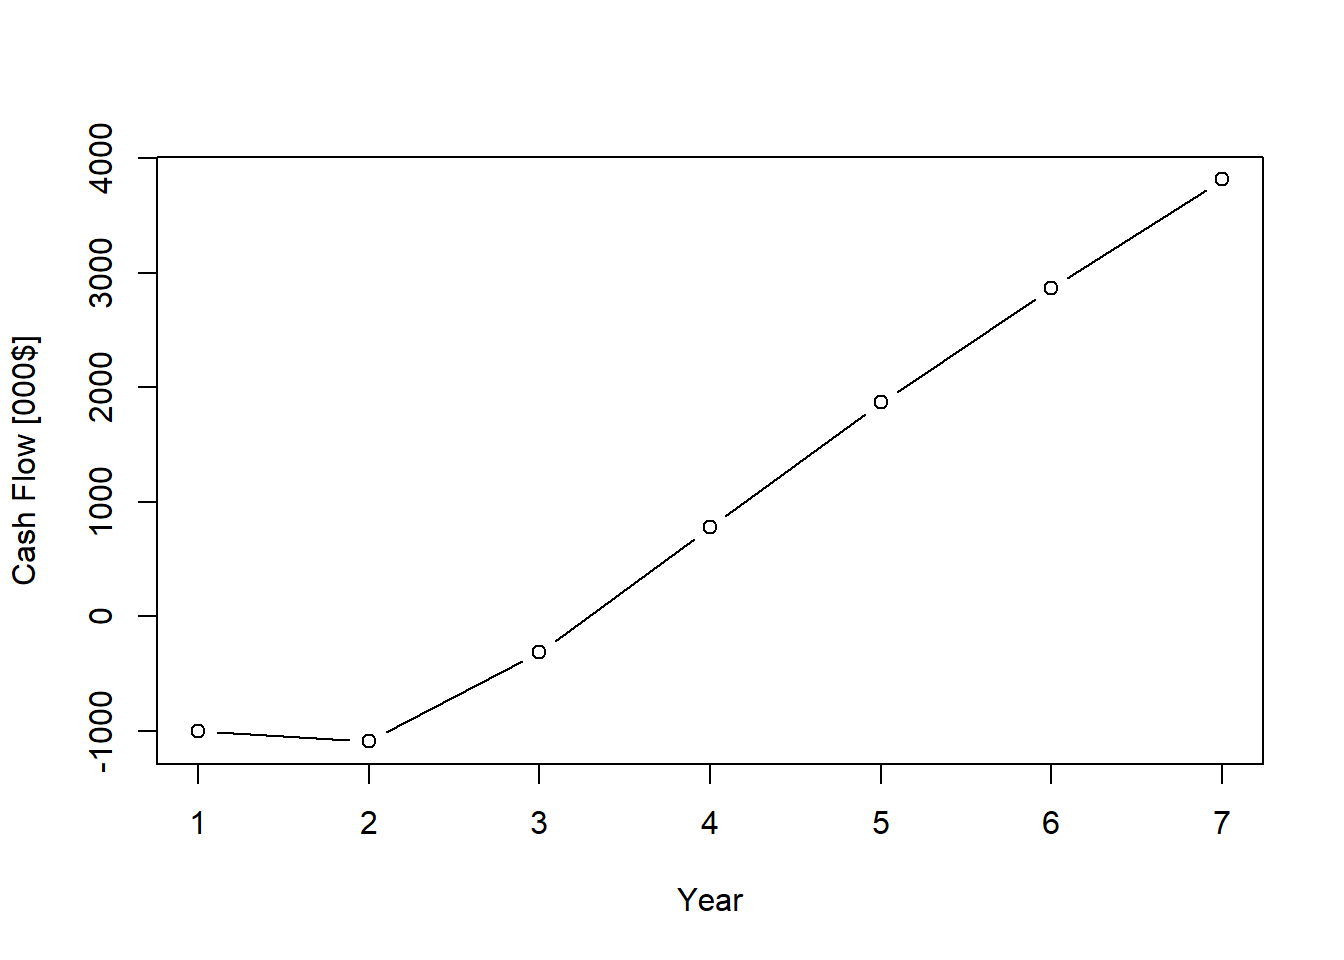
\includegraphics{2020-07-06-pre-seed-early-stage-saas-startup-business-modeling_files/figure-latex/unnamed-chunk-5-1.pdf}

\hypertarget{net-present-value}{%
\subsection{Net Present Value}\label{net-present-value}}

\begin{Shaded}
\begin{Highlighting}[]
\NormalTok{discount.factors <-}\StringTok{ }\DecValTok{1}\OperatorTok{/}\NormalTok{(}\DecValTok{1} \OperatorTok{+}\StringTok{ }\NormalTok{kDiscountrate }\OperatorTok{/}\StringTok{ }\DecValTok{100}\NormalTok{) }\OperatorTok{^}\StringTok{ }\NormalTok{year}
\NormalTok{discounted.cash.flow <-}\StringTok{ }\NormalTok{cash.flow }\OperatorTok{*}\StringTok{ }\NormalTok{discount.factors}
\KeywordTok{plot}\NormalTok{(year,}
\NormalTok{discounted.cash.flow,}
\DataTypeTok{xlab =} \StringTok{"Year"}\NormalTok{,}
\DataTypeTok{ylab =} \StringTok{"Discounted Cash Flow [$000]"}\NormalTok{,}
\DataTypeTok{type =} \StringTok{"b"}\NormalTok{)}
\end{Highlighting}
\end{Shaded}

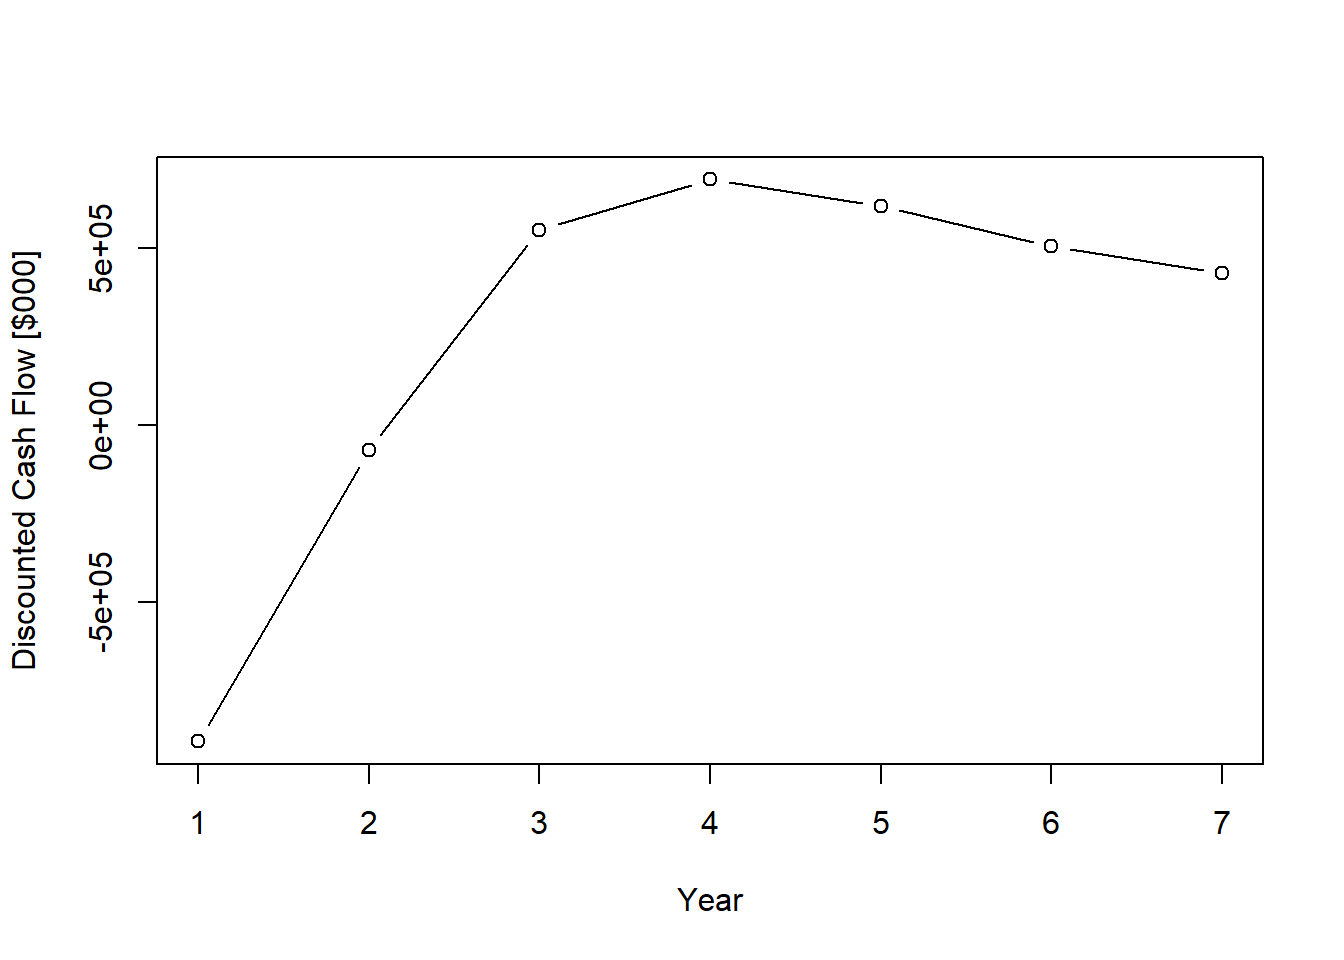
\includegraphics{2020-07-06-pre-seed-early-stage-saas-startup-business-modeling_files/figure-latex/unnamed-chunk-6-1.pdf}

\begin{Shaded}
\begin{Highlighting}[]
\NormalTok{npv <-}\StringTok{ }\KeywordTok{sum}\NormalTok{(discounted.cash.flow)}
\end{Highlighting}
\end{Shaded}

\textbf{Net Present Value is} \ensuremath{1.8341975\times 10^{6}}

\hypertarget{pro-forma-table-1}{%
\subsection{Pro Forma Table}\label{pro-forma-table-1}}

\begin{Shaded}
\begin{Highlighting}[]
\NormalTok{pro.forma.vars <-}\StringTok{ }\KeywordTok{array}\NormalTok{( }\KeywordTok{c}\NormalTok{(sales, revenue, gross.profit,}
\OperatorTok{-}\NormalTok{opex, }\OperatorTok{-}\NormalTok{depr, op.profit.before.tax, }\OperatorTok{-}\NormalTok{tax, op.profit.after.tax, depr, }\OperatorTok{-}\NormalTok{capex, cash.flow ), }\DataTypeTok{dim =} \KeywordTok{c}\NormalTok{(kHorizon, }\DecValTok{11}\NormalTok{))}
\NormalTok{pro.forma <-}\StringTok{ }\KeywordTok{data.frame}\NormalTok{(pro.forma.vars)}
\NormalTok{pro.forma.headers <-}\StringTok{ }\KeywordTok{c}\NormalTok{(}\StringTok{"Sales [breeding programs]"}\NormalTok{, }\StringTok{"Revenue"}\NormalTok{,}\StringTok{"Gross Profit"}\NormalTok{,}
\StringTok{"OPEX"}\NormalTok{, }\StringTok{"-Depreciation"}\NormalTok{, }\StringTok{"Operating Profit Before Tax"}\NormalTok{, }\StringTok{"Tax"}\NormalTok{, }\StringTok{"Operating Profit After Tax"}\NormalTok{, }\StringTok{"+Depreciation"}\NormalTok{, }\StringTok{"CAPEX"}\NormalTok{,}
\StringTok{"Cash Flow"}\NormalTok{)}
\KeywordTok{colnames}\NormalTok{(pro.forma) <-}\StringTok{ }\NormalTok{pro.forma.headers}
\KeywordTok{rownames}\NormalTok{(pro.forma) <-}\StringTok{ }\NormalTok{year}
\NormalTok{pro.forma =}\StringTok{ }\KeywordTok{t}\NormalTok{(pro.forma)}
\NormalTok{pro.forma}
\end{Highlighting}
\end{Shaded}

\begin{verbatim}
##                                  1             2             3       4       5
## Sales [breeding programs]    0e+00      16.66667      33.33333      50      50
## Revenue                      0e+00  850000.00000 1700000.00000 2550000 2550000
## Gross Profit                 0e+00  680000.00000 1360000.00000 2040000 2040000
## OPEX                         0e+00 -170000.00000 -340000.00000 -510000 -510000
## -Depreciation                0e+00 -250000.00000 -375000.00000 -375000 -375000
## Operating Profit Before Tax  0e+00  260000.00000  645000.00000 1155000 1155000
## Tax                          0e+00  -98800.00000 -245100.00000 -438900 -438900
## Operating Profit After Tax   0e+00  161200.00000  399900.00000  716100  716100
## +Depreciation                0e+00  250000.00000  375000.00000  375000  375000
## CAPEX                       -1e+06 -500000.00000       0.00000       0       0
## Cash Flow                   -1e+06  -88800.00000  774900.00000 1091100 1091100
##                                   6       7
## Sales [breeding programs]        50      50
## Revenue                     2550000 2550000
## Gross Profit                2040000 2040000
## OPEX                        -510000 -510000
## -Depreciation               -125000       0
## Operating Profit Before Tax 1405000 1530000
## Tax                         -533900 -581400
## Operating Profit After Tax   871100  948600
## +Depreciation                125000       0
## CAPEX                             0       0
## Cash Flow                    996100  948600
\end{verbatim}

\hypertarget{references}{%
\subsection{References}\label{references}}

The business model in this post based on a book by Robert D. Brown III
*Business Case Analysis with R**

\end{document}
